\documentclass{article}

\usepackage{amsmath}
\usepackage{amssymb}
\usepackage[russian]{babel}
\usepackage[14pt]{extsizes} % для того чтобы задать нестандартный 14-ый размер шрифта
\usepackage[left=20mm, top=15mm, right=15mm, bottom=30mm, footskip=15mm]{geometry} % настройки полей документа
\usepackage[style=gost-numeric]{biblatex}
\usepackage{graphicx}
\usepackage[utf8]{inputenc}
\usepackage{hyperref}

\usepackage{changepage}

%https://tex.stackexchange.com/questions/403463/signature-on-latex-lines
\newcommand\signature{%
   \begin{minipage}[t]{5cm}
   \vspace*{1.5ex}  % leave some space above the horizontal line
   \hrule
   \vspace{1mm} % just a bit more whitespace below the line
   \centering
   \begin{tabular}[t]{c}
   \small{(подпись)}
   \end{tabular}
   \end{minipage}}

\usepackage{xcolor}

\newcommand{\emptydate}{<<\underline{\phantom{99}}>> \underline{\phantom{февралиюня}} \the\year{} г.}

\addbibresource{citations.bib}

\title{Анализ игровых стратегий}
\author{Генералов Даниил}

\begin{document}

% НАЧАЛО ТИТУЛЬНОГО ЛИСТА
\begin{titlepage}
    \setlength{\parindent}{0cm}
    
    \begin{center}
    \hfill \break 
    \textbf{
    \normalsize{Федеральное государственное автономное образовательное учреждение высшего образования}\\
    \large{<<РОССИЙСКИЙ УНИВЕРСИТЕТ ДРУЖБЫ НАРОДОВ>>\\
    (РУДН)}
    }\\
    \normalsize{Основное учебное подразделение факультет физико-математических и естественных наук}\\ 
    \normalsize{Направление/специальность 09.03.03 <<Прикладная информатика>>}\\
    
    \vspace*{\fill}
    
    % \begin{flushright}
    % <<УТВЕРЖДАЮ>>
    
    % Заведущий кафедрой 
    
    % информационных технологий
    
    % д.ф.-м.н., проф.
    
    % \underline{\phantom{Ю.Н. Орлов}}Ю.Н. Орлов
    
    % \emptydate
    % \end{flushright}
    
    \Large{\textbf{ОТЧЕТ\\ о прохождении учебной практики\\ <<Научно-исследовательская работа\\ (получение первичных навыков научно-исследовательской работы)>>}}
    \\
    \tiny{(вид и наименование практики)}
    \\ \vspace{5mm}
    \normalsize{\underline{Генералов Даниил Михайлович}}
    \\
    \tiny{(Ф. И. О. обучающегося)}
    \vspace*{\fill}
    \end{center}
    
    Курс, группа \underline{3, НПИбд-01-21}

    Место прохождения практики \underline{
        <<Отдел технической поддержки пользователей ОТПП департамента технологических и информационных ресурсов РУДН и научные центры института компьютерных наук и телекоммуникаций РУДН>>
    }

    Сроки прохождения с <<15>> апреля 2024 г. по <<15>> июня 2024 г.

    \begin{adjustwidth}{0.5\textwidth}{0pt}
    Руководители практики:

    от РУДН \underline{Фомин М.Б., доцент  кафедры ММиИИ}

    от организации \underline{Самуйлов К.Е., директор ИКНиТ}
     
     \end{adjustwidth}
    
    Оценка: \underline{\phantom{1234567890 баллов}}
    
     
    \begin{center} \textbf{МОСКВА} \\ 2024 г. \end{center}
    \thispagestyle{empty} % выключаем отображение номера для этой страницы
     
    \end{titlepage}
     % КОНЕЦ ТИТУЛЬНОГО ЛИСТА
    
    \newpage


\section{Введение}

Согласно программе преддипломной практики направления подготовки 09.03.03 «Прикладная информатика» целями практики являются:
\begin{itemize}
\item формирование профессиональных навыков в проведении научных исследований;
\item формирование навыков использования современных научных методов для решения научных и практических задач;
\item формирование практических навыков написания вспомогательных программных комплексов для проведения вычислительных экспериментов;
\item формирование общекультурных, общепрофессиональный и профессиональных компетенций в соответствии с ОС ВО РУДН;
\item формирование навыков оформления и представления результатов научного исследования;
\item формирование навыков работы с источниками данных.
\end{itemize}

    Там же определены задачи практики:
\begin{itemize}
\item формирование у студентов навыков в области изучения научной литературы и (или) научно-исследовательских проектов в соответствии с будущим профилем профессиональной деятельности и применения новых научных результатов;
\item обучение правильному составлению научных обзоров и отчетов;
\item формирование навыков решения конкретных научно-практических задач самостоятельно или в научном коллективе;
\item обучение навыкам работы с прикладными комплексами программ для проведения вычислительных экспериментов;
\item формирование способности разработки вспомогательных программных инструментов;
\item обучение подготовке научных публикаций;
\item формирование способности проводить научные исследования и получать новые научные и прикладные результаты.
\end{itemize}

    Для достижения целей и решения поставленных задач в рамках преддипломной практики я выполнил обзор публикаций российских и международных научных изданий по теме выпускной квалификационной работы (ВКР) бакалавра, которая определена как <<Анализ игровых стратегий>>.

\newpage

\tableofcontents

\newpage

\section{Предварительная информация}

\subsection{История шахмат}

Шахматы -- одна из самых старых настольных игр, которая популярна до сих пор.
В близком к современному виду, шахматы существуют с 1475 годов~\cite{world_of_chess},
и начиная с XIX века они были стандартизированны организациями вроде Международной
Шахматной Федерации (ФИДЕ). Ввиду своей большой истории и высокой сложности, шахматы -- 
одна из самых глубоко анализированных игр. Из-за этого шахматы хорошо подходят 
как основа работы по анализу стратегических игр.

В базовом виде шахматы -- это игра для двух игроков,
которые выполняют один ход одной из фигур своего цвета. 
В начале игры фигуры располагаются на квадратной доске с 8x8 клетками,
где на второй и седьмой горизонтали расположены 8 пешек,
а на первой и восьмой -- остальные фигуры в определенном порядке.
Таковы правила ФИДЕ для международных шахмат~\cite{fide-laws},
но, как мы увидим, есть много вариантов игры,
в которых нарушаются каждое из этих правил.

\subsection{Компьютерные шахматы и другие стратегические игры}

Работа над разработкой автоматов, которые бы играли в шахматы,
велась ещё до изобретения цифровых компьютеров.
\footnote{Самое знаменитое устройство в этой сфере, так называемый <<механический турк>>~\cite{mechturk},
посредством иллюзионных приемов содержал человека-шахматиста,
и поэтому не считается настоящим автоматом.}
Но из-за механической природы они были очень ограничены в своих возможностях:
так, \emph{El Ajedrecista} -- автомат, который был построен в 1912 году~\cite{ajedrecista-article}
и реализовывал простой алгоритм~\cite{ajedrecista-algo}, который играет королем и ладьей
и всегда находит мат против одного короля.
Этот алгоритм можно описать всего сотней строк кода на языке программирования,
но из-за того, что это было реализовано электромеханически,
его размер был слишком большим,
чтобы таким образом реализовать какие-либо более сложные алгоритмы.

Самая ранняя компьютерная программа, которая играет в шахматы --
\emph{Turochamp}, которая была разработана в 1948 году 
и называется по именам своих двух авторов -- Алана Тьюринга и Дейвида Чамперновна~\cite{turochamp}.
Хотя Тьюринг не дожил до того времени, когда этот алгоритм можно было бы запустить на физическом компьютере,
он симулировал этот алгоритм вручную, чтобы играть против человека,
проиграв ему за 29 ходов,
где каждый из ходов вычислялся за 30 минут. 
Несмотря на это, этот алгоритм был успешно воплощен в компьютерных программах,
в том числе для веб-браузера~\cite{nimturochamp}.


Turochamp -- первая программа, которая использует алгоритм \emph{minimax},
который сейчас является основой большинства алгоритмов для игр с нулевой суммой
(то есть таких, что если один игрок выигрывает, то другой проигрывает).
Его базовая идея состоит в том,
что я хочу сделать позицию максимально выигрышной для себя,
а мой противник -- максимально проигрышной для меня.
Сначала определяется какая-то метрика, называемая \emph{evaluation},
которая выводит число, описывающее, насколько текущая позиция выигрышна.
Алгоритм рассматривает все возможные свои ходы из текущей позиции,
затем для каждой из результирующих позиций рассматривает возможные ответы противника,
и так далее ищет по дереву игры.
Когда ход у алгоритма, из этого дерева выбирается такой ход,
у которого evaluation \emph{макс}имальный,
а для ходов противника выбирается \emph{мин}имальный evaluation --
поэтому этот алгоритм называется \emph{minimax}.
После поиска выбирается такой из ходов,
который в перспективе дает наилучший evaluation,
даже если противник всегда выбирает лучший ход.

Из-за того, что в среднем количество возможных ходов в шахматной позиции
(так называемый \emph{branching factor})
в среднем около 30~\cite{chess-se-branching-factor},
делать полноценный поиск очень трудно:
уже после трех ходов (или 6 полуходов: один ход в шахматах состоит из одного полухода белых и одного полухода черных)
количество листовых ходов для рассмотрения составляет 729 миллионов.
Для того, чтобы сократить это количество,
используются различные эвристики: самая популярная из них называется \emph{alpha-beta pruning},
и она позволяет игнорировать те части дерева, которые не обещают никакого улучшения позиции.
Для этого хранятся два значения: \emph{alpha} и \emph{beta},
соответственно минимальный evaluation, который может получить тот игрок, который пытается максимизировать его,
и максимальный evaluation, который может получить тот игрок, который пытается минимизировать его.
С помощью этих значений алгоритм игнорирует все ветви,
в которых значение не будет меньше \emph{alpha} или больше \emph{beta}.
Это позволяет рассматривать гораздо меньшее поддерево всех возможных ходов,
размер которого в среднем составляет логарифм от размера исходного дерева.
Более того, такой алгоритм никогда не пропускает наилучший ход в данной позиции.

\subsection{Evaluation-функции}

Для того, чтобы такой алгоритм поиска работал правильно,
нужно иметь хорошую функцию оценки, или evaluation-функцию:
она принимает на вход позицию на доске и возвращает число,
которое качественно определяет степень,
в которой текущая позиция выигрышна.
Самые базовые функции используют в основном баланс \emph{материала} в позиции:
какие именно фигуры есть у одного и другого игрока.
Традиционное соотношение фигур и их ценности,
изначально приведенное в XVIII веке,
назначет пешке стоимость в один балл,
коню и слону -- 3 балла,
ладье -- 5 баллов
и ферзю -- 9 баллов.

Многие evaluation-функции также добавляют бонусы за \emph{мобильность},
чтобы фигуры предпочитали находиться в таких позициях,
где у них много доступных ходов.
Такие подходы называются \emph{hand-crafted evaluation} (\emph{HCE}),
потому что результирующая функция целиком сделана и настроена человеком.

Один из компонентов многих evaluation-функций является
так называемые \emph{piece-square tables} (<<таблицы фигур-клеток>>).
Это -- таблица, которая содержит число, которое описывает,
насколько предпочтительно каждому виду фигуры находиться на этой клетке~\footnote{
    Часто используют две таких таблицы: одну для дебютных позиций,
    а вторую для эндшпиля.
    В зависимости от материала на доске
    можно делать интерполяцию между двумя этими позициями,
    что дает возможность плавно варьировать стратегию.
}.

Такие таблицы могут быть написаны вручную,
чтобы закодировать базовые идеи:
например, таблица для пешек будет иметь одинаковые значения в каждой горизонтали,
которые повышаются от одного края доски к другому,
потому что пешкам стоит продвигаться в ферзи.
Аналогично, коням и ферзям стоит находиться в центре доски,
чтобы обеспечить наибольшую мобильность,
поэтому их таблица будет иметь приоритет к центру доски.

Эти таблицы также могут быть оптимизированны с помощью компьютерного поиска,
например алгоритмом вроде \emph{Texel's Tuning Method}~\cite{texel-tuning}.
Этот подход сначала собирает статистику из большого количества игр
между оптимизируемым движком и его предыдущей версией,
а затем использует степень ошибки для того, чтобы найти градиент каждого из параметров функции evaluation
и изменить его в соответствии с ним.
Такой процесс можно повторять несколько раз,
чтобы найти локальный минимум ошибки.

Улучшением этого подхода было использовать много piece-square tables
в зависимости от расположения короля на доске. 
Используя эту идею, в 2018 году Юу Насу предложил новую нейросетевую архитектуру,
названную \reflectbox{EUNN} (\emph{efficiently updatable neural networks})~\cite{nnue-paper}.
Такая нейросеть принимает на вход состояние доски и возвращает одно число -- evaluation
для текущей позиции.
Инновацией в этой архитектуре стала высокая степень параметризации входного слоя:
там есть несколько копий наборов нейронов, которые описывают позицию фигур на доске,
в зависимости от текущего положения королей на доске.
Как результат, большое количество нейронов входного слоя 
не используются для вычисления одной позиции,
и благодаря этому можно обновлять каждую долю этих нейронов без необходимости
обновлять все вместе --
это позволяет эффективно распределять эти вычисления на много разных компьютеров,
работающих над этим асинхронно.
Также, эта сеть разработана специально для оптимальной производительности
при расчете на CPU,
и скрытые слои имеют архитектуру, которая позволяет эффективно использовать SIMD-инструкции.
\reflectbox{EUNN}-сети были добавлены в Stockfish~\cite{stockfish} в версии 10 в 2018 году,
и благодаря этому Stockfish стал самым лучшим свободно-распространяемым шахматным движком~\cite{tcec-superfinal}.
Оптимизация, которая возможна с помощью нейросетей, быстро превысила пределы человеческого кода,
и в версии Stockfish 16.1 режим HCE был полностью удален.

\subsection{Человеческий анализ}

Описанный выше подход поиска хороших позиций в игровом дереве
эффективно работает для машин,
но он совсем не похож на то, как человек думает про шахматы.
Как говорят многие гроссмейстеры и международные мастера~\cite{benfinegold-blundering-short}~\cite{gothamchess-patterns},
шахматы -- это не игра интеллекта, а игра на распознавание образов:
преимущество будет у того игрока, который видел больше позиций, похожих на текущую. 

Из-за этого человеческие шахматисты уделают особенное внимание
изучению дебютов: если идет партия с определенным дебютом,
то скорее всего победит тот, кто изучил все возможные вариации на двадцать и больше ходов,
чем тот, кто видит это впервые.
В свою очередь, из-за этого популярны так называемые <<неправильные>> или <<иррегулярные>> дебюты,
которые по строгому анализу (и с точки зрения компьютеров) являются ошибочными~\cite{chessbase-chess-openings},
потому что это может сбить противника с его подготовленных вариаций и тем самым запутать его.

Компьютерный и человеческий анализ несовместимы и по другим причинам,
и одной из важных среди них являются ходы, которые сложно понять или объяснить.
Сначала это выражалось в так называемых <<анти-компьютерных тактиках,>>
получивших известность во время матча Каспаров---Deep Blue~\cite{kasparov-anti-computer-chess}.
Сначала требуется вывести компьютер из исследованной территории,
например посредством одного из <<неправильных>> дебютов,
которые не будут встречаться в его базе данных.
После этого, анти-компьютерный стиль игры подразумевает пассивные, стратегические ходы,
так чтобы противник не заметил план по улучшению своей позиции ввиду органиченной глубины поиска.
Так, если компьютер ищет позиции в глубину в 10 полуходов, а задуманная стратегия даст преимущество через
12-20 полуходов, то компьютер не сможет увидеть и обойти угрозу.
Напротив, классические приемы против человека, вроде <<ловушек>> на 2-3 хода,
не работают против компьютеров.

Сейчас, когда компьютеры играют неизмеримо лучше человека,
мы встречаемся с противоположной проблемой,
когда компьютер может сделать ход,
смысл которого человек не может понять.
Самый известный пример такой ситуации возник в матче между Ли Сидолом и AlphaGo,
компьютерной программой по игре в Го от Google.
В одной из игр компьютер сыграл знаменитый <<ход 37,>>
который сначала показался зрителям ошибкой,
но затем оказался решающим для всей игры~\cite{wired-alphago}.

Также, такие необъяснимые ходы часто используются для обнаружения
мошенничиства, особенно в онлайн-играх:
Stockfish~\cite{stockfish} -- свободно распространяемое ПО,
и поэтому кто угодно может использовать его в онлайн-играх,
чтобы находить лучшие ходы и тем самым жульничать.
Однако Stockfish (и другие компьютерные движки)
имеют свойство в сложных позициях выбирать такие ходы, которые человек не выбрал бы,
потому что они не выглядят связанными с тем, что происходит на доске,
и имеют очень далеко идущие идеи.
Если человек играет такой неожиданный ход, и этот ход при этом
является одной из топ-рекомендаций Stockfish,
то это очень хороший индикатор, что человек жульничает,
и это могут заметить как высокорейтинговые игроки~\cite{gothamchess-cheater-exposed},
так и автоматические процессы~\cite{lichess-kaladin}.

\subsection{Человекоподобные шахматы}

С тех пор, как Deep Blue победил Каспарова,
компьютеры играют в шахматы все лучше и лучше.
Stockfish сейчас на таком уровне,
что, согласно его рейтингу,
он победит всех гроссмейстеров в мире,
даже когда запущен на смартфоне.
У человека больше нет шансов победить против лучших компьютерных программ,
поэтому многие даже не пытаются.

В связи с этим требуются алгоритмы,
которые играют хорошо, но которые могут проиграть человеку данного уровня.
Это нужно, чтобы у человека были возможности учиться на живых примерах игры.
По такой же причине ИИ в компьютерных играх всегда разрабатываются
с какой-то слабостью~\cite{gmtk-ai}.

Один из таких проектов -- Maia Chess~\cite{maia-chess-article}~\cite{maia-chess-repo} -- 
состоит из нейросети, которая натренирована предсказывать ходы --
не обязательно самые лучшие, но самые вероятные от человека.
Был взят датасет игр Lichess~\cite{lichess-dataset},
отфильтрован по рейтингу,
и затем нейросеть использована для того, чтобы предсказывать ходы игроков,
в особенности храрактерные ошибки.
Из-за усреднения данных бот играет лучше, чем каждый из игроков отдельно взятый:
та версия бота, которая была натренирована на играх рейтинга около 1100,
играет против тех же игроков на уровне 1500\footnote{
    Учитывая такой результат, можно попробовать собрать много низкоуровневых игроков
    и предлагать им голосовать над возможными шахматными ходами,
    тем самым устраивая распределенный консультационный матч,
    и сравнить их общую эффективность с их отдельным результатом.
}.

Также можно использовать стандартные шахматные программы,
но ограничивать их в ресурсах.
Например, можно использовать настройки Stockfish,
которые ограничивают бюджет времени или позиций,
которые ему разрешено просматривать,
чтобы сделать его более легким для игрока.
У Stockfish уже есть встроенные настройки <<сложности,>>
которые делают что-то внутри алгоритма,
чтобы сделать его рекомендации менее качественными,
но более быстрыми.

В некоторых шахматных программах добавляются функции специально,
чтобы сделать их более интересными и менее сильными.
Например, Komodo~\cite{komodo-engine} имеет несколько <<персоналий>> --
опций, которые определяют, какие позиции он будет предпочитать: агрессивные,
оборонительные или эндшпильные (даже если сейчас не эндшпиль).
Эти настройки затем используются для создания интересных ботов для игроков:
например, Chess.com -- коммерческий шахматный сервер,
который предоставляет игрокам выбор разных ботов, с которыми можно играть.
Некоторые из ботов названы в честь известных шахматных игроков и знаменитостей,
и каждый имеет специальные настройки для Komodo, информацию о которых можно прочитать в~\cite{chesscom-bot-info}.
Целью этого является сделать ботов, которые имеют
выбранную сложность, при этом давая пользователям возможность
<<поиграть с своей любимой знаменитостью,>>
где реалистичность этого достигается путем настройки книги дебютов,
а также текстовых сообщений, которые боты пишут в ответ на определенные ходы.

Перспективная область исследования в этом направлении -- генеративные сети,
которые раньше успешно использовались для задач переписывания картинок в определенном стиле.
Предварительные исследования показывают, что они могут еще лучше симулировать стиль определенного игрока
и быть использованы в таких задачах, как боты Chess.com~\cite{chess-stylegan}.

\section{Шахматные варианты}

Ввиду своей долгой истории, было придумано много разных шахматных \emph{вариантов} --
игр, чьи правила основаны на шахматах, но отличаются от них в каких-то аспектах.
В этой части мы рассмотрим несколько таких вариантов, 
подчеркивая различия в правилах от стандартных шахмат
и обращая особенное внимание на то,
каким образом эти новые правила
сказываются на процесс принятия решений для людей и компьютеров.

\subsection{Chess960}

Также известный как <<шахматы Фишера>>, этот вариант
отличается от стандартных шахмат тем, что первая и восьмая горизонталь располагаются случайным образом,
сохраняя некоторые органичения (а именно что у короля должны быть ладьи на обоих сторонах и у каждой стороны должно быть два слона на разных цветах клетки) --
в результате этих ограничений, всего могут быть 960 начальных позиций.
Этот вариант был изобретен чемпионом мира Бобби Фишером в 1992 году~\cite{chess960}
в ответ на наблюдение, что игра в шахматы начала становиться скучной
из-за того, что гроссмейстеры заучивали дебюты 
и все игры были предсказуемыми.

Благодаря большому количеству начальных позиций, 
которые выбираются непредсказуемо (иногда даже полностью случайно),
выучить дебюты для каждой из этих начальных позиций
не представляется возможным.
Поэтому игрокам нужно опираться на базовые шахматные правила,
вроде выдвижения коней и слонов, контроля центра доски пешками,
а также защита короля:
последнее может быть сложно, потому что, в зависимости от расположения ладьей,
может не быть настолько защищенного места для рокировки, как в стандартных шахматах.
Так, если рокировка выводит короля к центру доски, а не к краю, то скорее всего ее не стоит делать.

\subsection{Бесконечные шахматы}

Этот вариант отличается от обычных шахмат тем, 
что доска не ограничена по высоте и ширине,
и фигуры могут двигаться выше восьмой и ниже первой горизонтали,
левее вертикали A и правее вертикали H.
Как следствие этого правила, пешки не могут быть продвинуты в другие фигуры, потому что нет границы, до которой они должны были бы продвинуться;
также отключаются правила \emph{взятия на проходе} и рокировки.

Бесконечные шахматы -- это обычно не игра, в которую играют люди, --
вместо этого это математическая структура, в которой можно находить интересные факты:
например, тот факт, что существуют такие позиции,
в которых гарантированна победа только в случае, когда игроки следуют
детерминистичной и вычислимой стратегии, а если снять это ограничение, то возможна ничья~\cite{transfinite-game-values} 
(что подтверждает теорему об ограниченности Тьюринг-машин без оракулов),
или тот факт, что задача о нахождении мата в $n$ ходов 
является решаемой для бесконечных шахмат~\cite{infinite-mate-in-n}
(что значит, что такая задача для обычных шахмат может иметь похожее решение).

\subsection{Аримаа}

Эту игру изобрел Омар Саед в 2003 году в реакцию на поражение Гарри Каспарова против Deep Blue~\cite{arimaa}.
Целью было разработать такую игру, которая была бы сложна для компьютеров,
но при этом понятна и интересна для людей (в частности для его четырехлетнего сына Аамира -- в его честь и названа игра),
а также чтобы в нее можно было играть с помощью шахматной доски и фигур.

Игра начинается с того, что оба игрока располагают свои фигуры (одного слона, одного верблюда, двух коней, двух собак, двух кошек и восемь кроликов)
в любом порядке на своих двух горизонталях.
После этого каждый из игроков делает от одного до четырех действий за ход,
двигая свои фигуры вперед, влево, вправо и (за исключением кроликов) назад.
Более сильные фигуры могут тянуть и толкать более слабые фигуры противника,
а фигуры, рядом с которыми стоит более сильная вражеская фигура, не могут двигаться.
Фигуры не могут взять другие фигуры сами по себе,
вместо этого они должны быть сдвинуты на одну из четырех <<ловушек>>,
которые находятся на клетках C3, F3, C6 и F6.
Если фигура находится на этой клетке, и рядом с ней нет союзных фигур,
то она удаляется из игры.
Чтобы победить, игрок может либо продвинуть своего кролика до противоположной горизонтали
(как в шахматах пешки продвигаются в другие фигуры),
либо сделать так, чтобы у противника не было доступных ходов,
либо вывести из игры всех кроликов противника.

Эта игра сложнее для компьютеров, чем шахматы.
Во-первых, фактор ветвления здесь больше:
можно за один ход сделать одно, два, три или четыре действия,
но они происходят друг за другом (так как одно действие может сделать другое невозможным),
и из-за этого их необходимо рассматривать в цепочке.
Более того, этот фактор ветвления не сокращается, как в шахматах:
взятие фигур происходит гораздо меньше,
и это значит, что здесь нет <<эндшпиля>> в шахматном виде,
где остается совсем небольшое количество фигур,
для которых можно быстро посчитать путь до победы.

Тем не менее, в 2015 году был разработан алгоритм, который смог победить другие программы
и людей в этой игре. Его автор написал статью~\cite{arimaa-program}, в которой
он рассказывает, что многие из используемых функций похожи на те,
которые используются в шахматных алгоритмах (alpha-beta pruning, killer move heuristic, quiescence search итд.),
но многие специфичны для Аримаа (trap control, hostages, elephant mobility, frames итд.).

\subsection{5D Chess with Multiverse Time Travel}

Этот шахматный вариант реализован в виде компьютерной игры, выпущенной в 2020 году~\cite{5dchess-steam}.
Стандартная шахматная игра расширяется дополнительным измерением времени (позиция на доске сейчас может влиять на позицию, которая была раньше)
и параллельными линиями времени (фигуры могут сдвинуться назад во времени, создавая новую версию истории)\footnote{
    Это значит, что, строго говоря, 5D Chess -- на самом деле четырехмерная игра,
    и название слегка преувеличено.
}.
Разработчик взял каждую фигуру и дополнил ее движение в новых измерениях: 
например, в стандартных шахматах ладья двигается ортогонально по вертикали и горизонтали,
поэтому в 5D Chess, когда она двигается по времени, она остается на том же положении на доске;
аналогично, король может сдвинуться на один шаг в любом направлении, в том числе вперед и назад по времени
и на один шаг между линиями времени.

Ввиду необходимости хранить всю историю игры в активном использовании,
в 5D Chess невозможно играть на физических шахматных досках.
Более того, даже на компьютере, необходимость хранить историю в памяти
значит, что эта игра очень сложная для понимания человеком~\cite{5dchess-review}.
В игре встроены несколько головоломок, которые объясняют правила,
и решения часто очень неинтуитивны:
например, ладья очень часто может поставить мат королю в прошлом,
даже если на текущей доске этот ход даже не является шахом,
потому что критерием победы является поставить мат любому из королей на всех досках.
Есть случаи, когда в играх между начинающими игроками,
один из них ставит мат другому, не зная этого,
и как результат оба игрока не понимают, что произошло~\cite{5dchess-rtgame}.

Дизайн игры делает ее слегка более простой для компьютеров, но не слишком.
В обычных шахматах размер состояния игры ограничен и не велик
(так, в модуле \texttt{shakmaty}~\cite{shakmaty-crate} в Rust размер структуры \texttt{Chess} составляет 136 байтов,
и он может быть оптимизирован еще больше с потерей производительности),
в то время как в 5D Chess создается неограниченное количество состояний шахматной доски:
как минимум одна создается каждый ход,
и необходимо хранить все из них
(потому что почти всегда существует последовательность ходов,
которая вернет время вспять до любой отдельной доски на основной линии времени).
Из-за этого потребность в памяти растет по мере игры (или поиска по дереву),
количество возможных ходов увеличивается в зависимости от количества шагов времени, которые существуют до и после одной доски,
и сложность функции evaluation также растет как минимум квадратично с количеством текущих активных досок.
Несмотря на это, компьютеры имеют значительное преимущество против человека в том,
что они не забывают о том, что происходило несколько досок назад.
Помимо этого довольно сложно судить о сложности игры,
потому что ей не было уделен такой же уровень внимания, как стандартным шахматам,
и это усугубляется степенью контринтуитивности игры. 

\subsection{Шахматы с тремя игроками}

Существует семейство вариантов,
которые подразумевают больше чем двух игроков
(чаще всего 3).
Некоторые такие варианты используют квадратные клетки,
но большинство выбирают доски с другой ячейкой,
например треугольные или шестиугольные клетки.

Добавление третьего игрока делает так, что игра больше не имеет нулевую сумму,
как стандартные шахматы:
теперь у третьего игрока есть интерес в том, что происходит между двумя другими.
Это значительно меняет их поведение.
Например, есть варианты, когда выигрывает тот игрок, кто поставил мат,
а проигрывает и тот, кому поставлен мат, и третий, -- 
тогда каждый игрок должен не только защищать себя, но также мешать двум другим игрокам поставить мат друг другу.
Аналогично, игроки будут обменивать меньше фигур,
потому что при обмене у первого и второго игрока становится меньше материала,
а у третьего он сохраняется.

Двое игроков могут сговориться против третьего, если правилами игры это выгодно,
и вытеснить его из игры, прежде чем сражаться между собой.
Для этого некоторые варианты, вроде запатентованного Ильшатом Тагиевым~\cite{triad-chess},
вводят \emph{<<правило нейтралитета>>}:
игрок 3 может нападать на игрока 2, только если 2 нападал на 3 на предыдущем ходу,
или если 1 не нападал на 2. 
Как результат этого правила, двое игроков не могут скоординировать атаку на третьего,
если третий не даст им возможность на это. 
Как следствие этого, для компьютерного анализа нельзя будет применять \emph{NegaMax} --
стандартную оптимизацию, которая говорит, что если для одного игрока есть преимущество в +5 очков,
то другой игрок имеет отрицательное преимущество в -5 очков -- 
из-за того, что есть три игрока, у каждого из которых свое положение армий,
нельзя просто так отрицать evaluation одного игрока, 
чтобы получить evaluation другого.

Как человеческий, так и компьютерный анализ осложняется тем, что нужно продумывать больше времени вперед:
требуется расчитать возможный ход одного и другого противника, а также
вопрос о том, кто будет атаковать кого на этот ход. 
Эти два фактора увеличивают пространство поиска примерно в четыре раза. 
Любые дебюты должны разрабатываться с взглядом на тот фактор,
что они должны быть адаптируемы к возможностям атаки на обе стороны,
и из-за этого особенно важными становятся слоны и ладьи,
потому что они могут двигаться на любое расстояние за ход,
и поэтому, находясь в центральном положении,
могут быстро переключить атаку с одного противника на другого.


\subsection{Kung-Fu Chess}

Этот вариант был разработан в 2000х годах
и получил награду зрителей на Фестивале Независимых Игр в 2002 году~\cite{igf-kungfuchess}.
Этот вариант может быть реализован только на компьютере с интернет-соединением,
а не на физической доске,
и после закрытия официального сервера игры в 2008 году
появились много альтернативных~\cite{kfchess}.

Суть этого варианта заключается в том, 
чтобы игра проходила в реальном времени,
без разделения на ходы. 
Вместо этого, каждая фигура может двигаться в любой момент,
с задержкой после каждого хода.
По изначальной задумке, это должно сделать шахматы более похожими на
RTS-игры, вроде StarCraft и Dota 2.
Из-за этого тайминг становится критичным,
потому что от того, когда именно была отправлена команда сдвинуть фигуру,
будет зависеть, сможет ли вражеская фигура взять ее.

У компьютера в такой игре абсолютное преимущество:
в отличие от человека, компьютер может не только расчитать хороший шахматный ход лучше чем человек,
но и определить, когда именно выполнить его, чтобы помешать планам человека.
Помимо этого, как и в обычных RTS, в Kung-Fu Chess
компьютер имеет преимущество в том, что он может видеть все что происходит на доске одновременно,
в то время как человек должен переводить внимание (и курсор мыши) с одной стороны на другую.
Учитывая это преимущество,
большинство алгоритмов для Kung-Fu Chess 
имеют встроенные ограничения,
чтобы против них было возможно выиграть -- 
как и большинство ИИ для компьютерных игр.
Например, они имеют ограничения,
которые мешают им выводить своего короля из под атаки
или сразу атаковать короля противника,
хотя это может стоить им всей партии.

\subsection{Шведские шахматы}

Также известные как <<bughouse chess>> или <<шведки,>>
в этот вариант играют двое против двоих людей на двух досках,
которые расположены противоположно друг другу,
так что один игрок на команде играет белыми фигурами, а другой -- черными.
Когда игрок белыми фигурами берет вражескую черную фигуру, он передает ее
своему союзнику в запас.
Затем, на свой ход, вместо того чтобы двигать свою фигуру,
игрок с черными фигурами может взять одну фигуру из запаса и поставить ее на свободное место на доске.
Помимо этого, если один игрок продвигает пешку на последнюю горизонталь,
то он может в этот момент произвести снятие, забрав любую из фигур противника с тем же цветом и оставив ему пешку в резерве.

В классической интерпретации, ходы происходят асинхронно между двумя досками.
Это значит, что иногда одному игроку бывает полезно <<зависнуть>>
в ожидании изменений на другой доске.
Из-за этого очень важна коммуникация, где игроки смотрят за состоянием на другой доске
и дают советы, какие фигуры они хотели бы получить в запас. 
В таких ситуациях, иногда бывает полезно играть сверх-агрессивно,
намеренно теряя фигуры,
просто чтобы получить вражеских фигур, чтобы передать на другую доску.
Помимо этого, фигуры в резерве становятся намного ценнее, чем фигуры на доске ввиду своей повышенной мобильности:
в частности, пешки становятся очень ценны,
потому что с помощью них можно дешево заблокировать две клетки,
а также их можно поставить на предпоследнюю (не последнюю) горизонталь и тем самым быстро получить возможность снятия с другой доски.

При разработке алгоритма для игры в шведки нужно учитывать не только состояние на доске
и не только фигуры в резерве,
но также и потенциальные будущие события на другой доске,
которые могут привести к появлению новых фигур.
В случае разработки алгоритма, который бы играл в кооперации с человеком,
нужно иметь возможность передавать ему свои намерения,
а также просить его сделать определенные маневры,
вроде взятия определенных фигур и зависания в ожидании снятия.

Есть вариант шведских шахмат, в которые играют два игрока -- <<Crazyhouse,>>
в которых взятие фигур противника ставит их в свой собственный резерв (с противоположным цветом).
В этот вариант легче играть на компьютере, потому что в реальном мире фигуры не могут менять цвет, когда они переходят в запас.
Этот вариант также легче для обработки компьютером, потому что он не требует
коммуникации с другой доской;
он тогда действует лишь как обычные шахматы с повышенным количеством ходов (в частности с возможностью поставить каждую из фигур запаса на каждую из свободных клеток).
Поскольку фигуры никогда не заканчиваются,
основные знания про шахматный эндшпиль также становятся бесполезными,
из-за чего, как в Аримаа, глубокий анализ игры будет трудным на каждом этапе игры.
Помимо этого, фигуры в запасе будут делать анализ сложнее,
потому что чем больше фигур в запасе, тем больше потенциальных ходов, которые связаны с ними,
поэтому довольно эффективной стратегией против слабых ИИ-противников может быть сохранять как можно больше фигур в запасе,
чтобы держать branching factor высоким.

\section{Шахматы со сливающимися фигурами: Chessplus}

В этой части мы рассмотрим шахматный вариант,
который представил наибольший интерес для автора этого отчета.
В контексте этого варианта была проделана разработка ПО,
которое также будет представлено в этой части.

\subsection{Chessplus}

В 2020 году австралийская семья организовала компанию по продаже новой настольной игры под названием <<Chessplus.>> 
Согласно сайту~\cite{chessplus-site}, идея для этой игры пришла, когда девятилетняя дочь создателя использовала противоправную комбинацию пешки и ладьи,
чтобы получить ферзя и победить в шахматах против ее отца.
Игра была построена вокруг того, чтобы такое действие было разрешено.

В эту игру играют на обычной шахматной доске,
используя стандартные шахматные фигуры необычной формы\footnote{
    Основная бизнес-модель этой компании -- продажа шахматных наборов, которые имеют эту необычную форму.
}.
Эти фигуры могут стоять отдельно, а могут быть соединены вместе с другими, 
и вокруг этого построены правила.

В свой ход, игрок может взять любую отдельно стоящую фигуру
и сдвинуть ее на клетку, где уже стоит другая отдельно стоящая фигура (любая, кроме короля).
Как результат этого, в клетке назначения становится фигура, которая состоит из двух частей.
После этого, комбинированная фигура может двигаться вместе,
соответствуя правилу для любого из его компонентов.
В свой ход комбинированная фигура также может разделиться на свои компоненты:
одна половина двигается, а другая остается на предыдущем месте.
(Двигающаяся половина может в результате хода также присоединиться к другой фигуре.)
Если противник берет комбинированную фигуру, то обе ее части удаляются из игры;
аналогично, если комбинированная фигура, которая содержит пешку, доходит до последней горизонтали,
то обе части удаляются из игры, а на этом месте появляется единичный ферзь\footnote{
    По всей видимости, по правилам не разрешено продвижение в фигуры кроме ферзей:
    на продаваемых комплектах написано только то, что в них содержатся дополнительные ферзи,
    и официальное приложение подразумевает только продвижение в ферзя,
    и инструкция~\cite{chessplus-rules} указывает только на возможность продвижения в ферзей.
}.

Есть официальные названия комбинированных фигур,
которые являются комбинацией их обычных названий.
В каждом из них вперед ставится фигура,
которая идет раньше в этом списке:
queen, bishop, knight, rook, pawn (это сделано для благозвучия: \emph{knook} а не \emph{roight}
\footnote{
    В инструкции к игре 2016 года~\cite{chessplus-rules} используются другие названия, которые
    ставят фигуры в другом порядке очередности: queen, rook, knight, bishop, pawn.
    Из-за этого там появляются другие варианты названий,
    например \emph{roawn}, \emph{roight}, \emph{knishop} и \emph{biawn}.
    Рядом с этими названиями также написан знак незарегестрированной торговой марки,
    из-за чего использование этих названий может быть проблематично.
}).
В скобках приведен примерный перевод этих названий.

\begin{itemize}
    \item DQueen -- queen+queen (двойной ферзь)
    \item Quishop -- queen+bishop (ферслон)
    \item Quight -- queen+knight (ферконь)
    \item Quook -- queen+rook (ферладья)
    \item DBishop -- bishop+bishop (двойный слон)
    \item Bight -- bishop+knight (слоноконь)
    \item Biook -- bishop+rook (слоноладья)
    \item Biawn -- bishop+pawn (слонопешка)
    \item DKnight -- knight+knight (двойный конь)
    \item Knook -- knight+rook (конеладья)
    \item Knawn -- knight+pawn (конепешка)
    \item DRook -- rook+rook (двойная ладья)
    \item Roawn -- rook+pawn (ладьепешка)
    \item DPawn -- pawn+pawn (двойная пешка)
\end{itemize}

\subsection{Особенности стратегий}

Согласно создателям игры, эта игра более проста в изучении и более интересна, чем обычные шахматы,
потому что здесь не требуется выдвижение пешек, чтобы открыть пространство для движения других фигур.
Действительно, эта особенность делает игру более быстротечной в дебюте,
потому что можно за один ход расположить слона на диагонали, где он будет видеть много перспективных клеток,
просто комбинируя его с одной из пешек.

Из-за того, что полная комбинированная фигура заменяется на ферзя при продвижении,
предпочтительно использовать комбинацию, чтобы доставить пешку на предпоследнюю горизонталь,
а затем сделать один ход пешкой, чтобы избежать потери материала.
Противник может баррикадировать эту пешку, чтобы она не смогла достичь последней горизонтали (как и в обычных шахматах),
но здесь эта баррикада будет относительной:
поскольку ладьи являются хорошим способом доставить пешку на предпоследнюю горизонталь,
и ладья, в отличии от пешки, может брать вертикально вверх, 
у нападающего игрока есть вариант обменять пешку с ладьей на ферзя,
тем самым получая меньшее преимущество в материале,
или же потратить несколько ходов: сначала взять защищающуюся фигуру отдельной ладьей, затем отодвинуть ладью куда-то (в том числе обратно на клетку с пешкой),
а затем продвинуть пешку на последнюю горизонталь.

Комбинация пешки и слона может быть очень полезной,
потому что пешка дает слону возможность сменить свою полярность;
в обычных шахматах, если один из слонов был взят,
то король может бесконечно избегать шаха от другого слона,
если остается только на клетках другого цвета.
С помощью комбинации пешки и слона можно сдвинуть его на другой цвет клетки,
что позволяет превращать белопольного слона в чернопольного (и наоборот).
К тому же, из-за того, что слон может двигаться назад,
эта пешка позволяет делать такой переход полярности бесконечно.

Комбинировать пешку с ферзем возможно, но это полезно только очень ситуативно:
ферзь может атаковать все те же клетки, как и пешка,
а продвижение пешки вместе с ферзем лишь потеряет пешку.
Наиболее полезно это делать для доставки пешки на предпоследнюю горизонталь (но для этого также подходит ладья, как описано выше),
или же для того, чтобы организовать защиту ферзя, когда он отделяется на одну клетку диагонально и ставит мат.

Комбинация ферзя и коня -- самая сильная из возможных комбинированных фигур.
Она закрывает недостатки ферзя,
который в обычных шахматах может быть атакован конем,
которого невозможно сразу взять. 
Наличие коня закрывает пробелы в покрытии клеток ферзем,
и на пустой доске это сочетание покрывает полный квадрат радиусом 2 клетки,
и в итоге это покрывает больше половины доски (35 клеток, не включая свою собственную).

\begin{figure}[h]
    \centering
    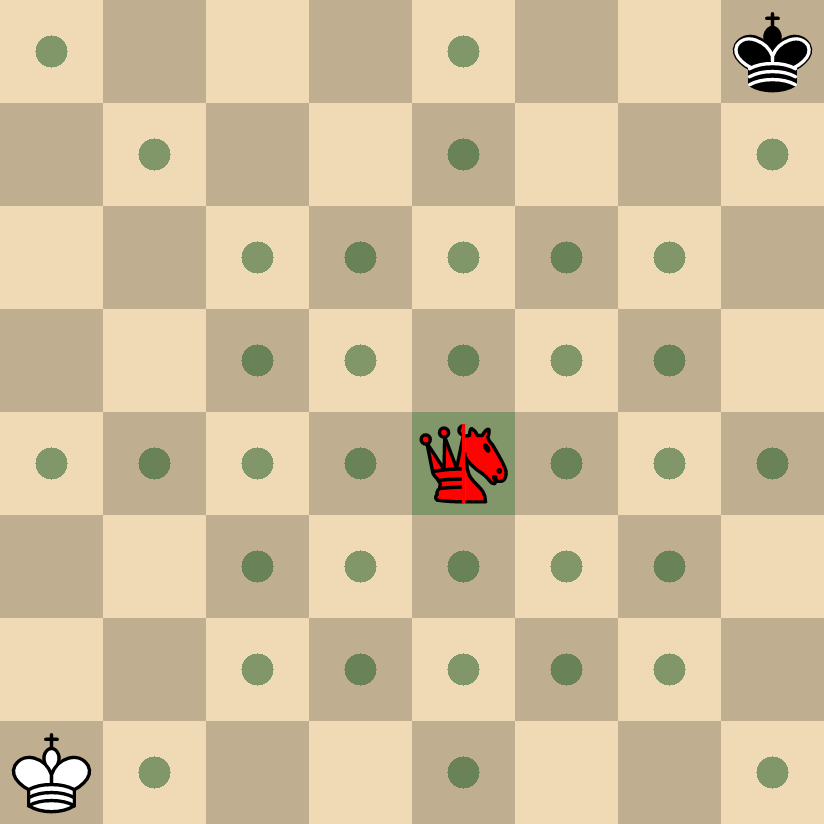
\includegraphics[width=0.5\textwidth]{img/queen-knight-demo.png}
    \caption{Комбинация ферзя и коня покрывает большую часть доски}
\end{figure}


Каждая фигура может соединяться с другой фигурой,
сделав свой стандартный ход,
и у большинства фигур (за исключением пешек)
есть возможность двигаться назад.
Учитывая это, каждая фигура может защищать сама себя:
если вражеская фигура угрожает этой клетке,
то одна из половинок фигуры может отделиться,
сделать любой ход,
и как результат она защищает исходную клетку.
Это дает возможность превратить ситуации безусловной потери материала в размен фигур.

\subsection{Реализация на компьютере}

Важным результатом этой работы является прототип реализации игры Chessplus
на компьютере.

Создатели игры опубликовали Android-приложение,
которое реализует эту игру,
но это приложение имеет недостатки:
для него не опубликован исходный код,
что делает трудным работу над этим проектом для других,
а тот факт, что это только Android-приложение
(а не веб-приложение),
требует доступа к смартфону или планшету, чтобы его использовать.

Для реализации были взяты элементы из Chessground~\cite{lichess-chessground} --
компонента сайта Lichess, который показывает пользователю шахматную доску.
Сначала была попытка использовать их код,
но ввиду недостаточного опыта работы с TypeScript,
вместо этого мы реализовали необходимую логику в Rust
с использованием Yew~\cite{yewstack-yew} -- фреймворка для разработки веб-приложений
с концепцией, похожей на React.

Взят набор фигур, изначально разработанный для демонстрации шахматных досок на Википедии~\cite{cburnett-pieces},
которые также используются как стандартный набор фигур на Lichess.
Эти фигуры доступны под лицензией GPDL,
а код Lichess и модуля \texttt{shakmaty}~\cite{shakmaty-crate} -- под GPLv3,
поэтому итоговый совокупный код также доступен под GPLv3.

Фигуры были вручную отредактированы, чтобы сделать версии,
которые содержат два конца,
посредством разделения фигуры вертикально на две половины,
а затем симметричного копирования их.
Так, двойной конь нарисован как конь с двумя головами,
разделенными посередине линией.
Эти картинки затем используются при визуализации шахматной доски.

\begin{figure}[h]
    \centering
    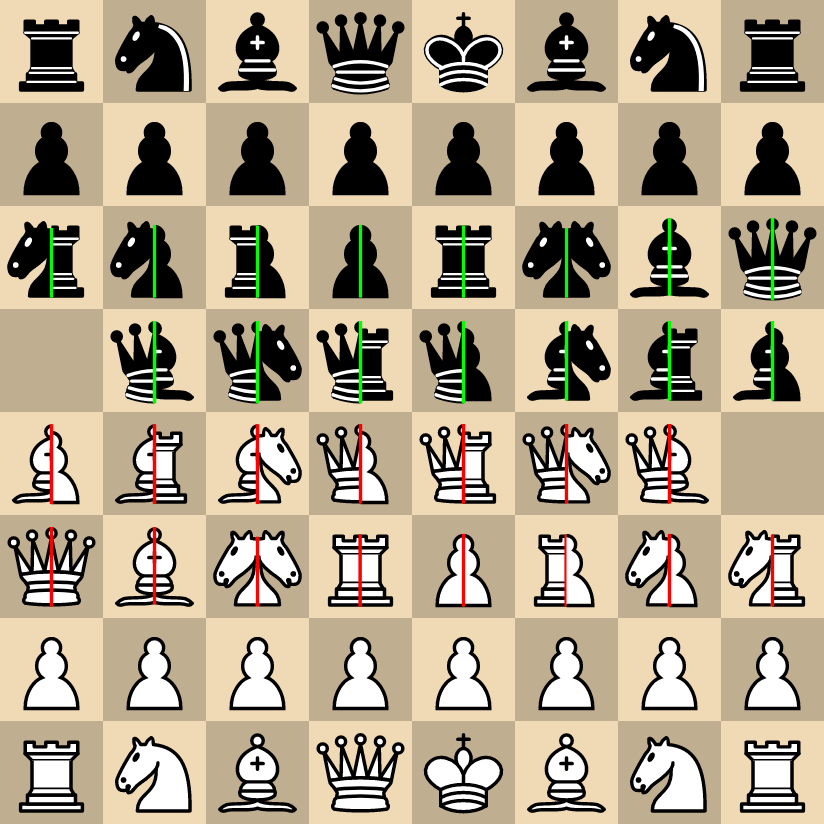
\includegraphics[width=0.5\textwidth]{img/all-pieces-demo.png}
    \caption{Все возможные фигуры, включая шесть стандартных в стартовой конфигурации и 15 возможных комбинаций}
\end{figure}


Из-за ограниченного времени, реализация логики перемещения фигур была сделана 
в том же самом модуле, как и сам компонент доски.
Правильный дизайн (как в Chessground) подразумевает разделение ответственностей,
чтобы компонент визуализации не содержал шахматной логики,
но в интересах простоты реализации эти вещи были объединены. 

Работа над реализацией была начата до того, как мы узнали про
существование свободно-доступной книги правил~\cite{chessplus-rules} и Android-приложения,
поэтому некоторые аспекты нашей реализации отличаются.
Например, в нашей реализации, пешки могут соединяться с другими фигурами посредством диагонального шага,
как будто они выполняют взятие этой фигуры --
это невозможно в Android-приложении, где пешки могут соединиться с другими фигурами
только вертикально вверх.
Текстовая инструкция не указывает, как именно такой ход разрешается выполнять.

\begin{figure}[h]
    \centering
    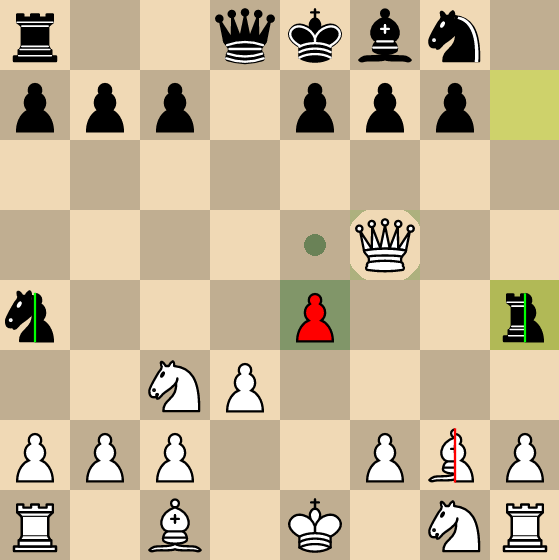
\includegraphics[width=0.5\textwidth]{img/diagonal-merging-question.png}
    \caption{В этой позиции, может ли белая пешка на e4 соединиться с ферзем на g5? В нашей версии да, в Android-приложении нет}
\end{figure}

Мы считаем Android-приложение авторитетным источником правил,
но в некоторых аспектах оно расходится с текстовой инструкцией.
Например, там совсем не реализовано взятие на проходе,
хотя в книге правил это упомянается, но с неоднозначностями.
В нашей версии взятие на проходе реализовано следующим образом:
если фигура, содержащая пешку (в том числе только пешка)
находится на пятой горизонтали относительно своей стороны,
и противник делает ход, который двигает фигуру, содержащую пешку,
с исходной горизонтали на две вверх,
то эту фигуру можно взять на проходе в этот ход.

\begin{figure}[h]
    \centering
    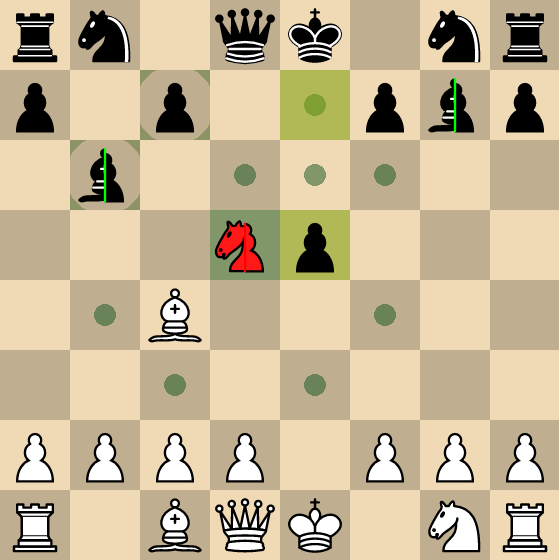
\includegraphics[width=0.5\textwidth]{img/enpassant-demo.png}
    \caption{
        В этой позиции черный игрок только что сыграл пешкой e7-e5. У белого игрока есть конепешка на d5.
        Только на этом ходу, белый игрок может взять эту пешку на проходе
        двумя способами: либо комбинированной конепешкой (KPdxe6 e.p.),
        либо отделив пешку от коня (dxe6 e.p.).
    }
\end{figure}


\section{Дальнейшая работа}

В этой работе мы рассмотрели множество различных шахматных вариантов,
и в частности то, как они влияют на выбор стратегий.
Мы также представляем компьютерную (а именно веб-)версию шахматного варианта,
который основан на сливании нескольких шахматных фигур вместе --
мы успешно реализовали интерфейс для игры,
а также алгоритм, который пытается выполнять alpha-beta поиск (но делает это очень медленно).

Для дальнейшего улучшения требуется найти оптимизированную структуру в памяти для доски,
которая подразумевает соединение фигур.
Для этого нужно адаптировать один из стандартных подходов, основанных на \emph{bitboards} --
именно такие используются в модуле \emph{shakmaty}~\cite{shakmaty-crate}.
Из него уже взят некоторый код,
поэтому будет удобно взять его для дальнейшей работы.

Чтобы сделать быстрый и эффективный алгоритм поиска качественных ходов,
нужно использовать больше функционала из топ-программ.
К сожалению, они часто зависят от большого количества эмпирических данных
про уже сыгранные игры
(например для оптимизации piece-square tables и \reflectbox{EUNN}-сетей).
Существует открытый датасет игр классических шахмат от Lichess~\cite{lichess-dataset},
в котором также есть несколько малых датасетов игр в популярные варианты,
но эти игры нельзя использовать как примеры игры в Chessplus.
Для сбора информации об играх может быть полезно сделать публичный сервер,
на котором можно играть в эту игру.


\newpage

\section{Список литературы}

\printbibliography

\end{document}